\section{Experiments}
In this section, we perform an extensive series of experiments aimed at evaluating the capabilities of \ourshort across various aspects, including navigation and manipulation. Specifically, our primary experiments are designed to: (1) verify the efficacy of \ourshort in efficiently and robustly transforming diverse human motion data into robot-plausible behaviors; (2) exhibit the effectiveness of our method in sim2real transfer; (3) quantify the accuracy and reliability of our navigation localization approach; (4) demonstrate the effectiveness of \ourshort in mobile manipulation. 

\subsection{Sample Efficiency of \ourshort}
\begin{figure*}[t]
  \centering
  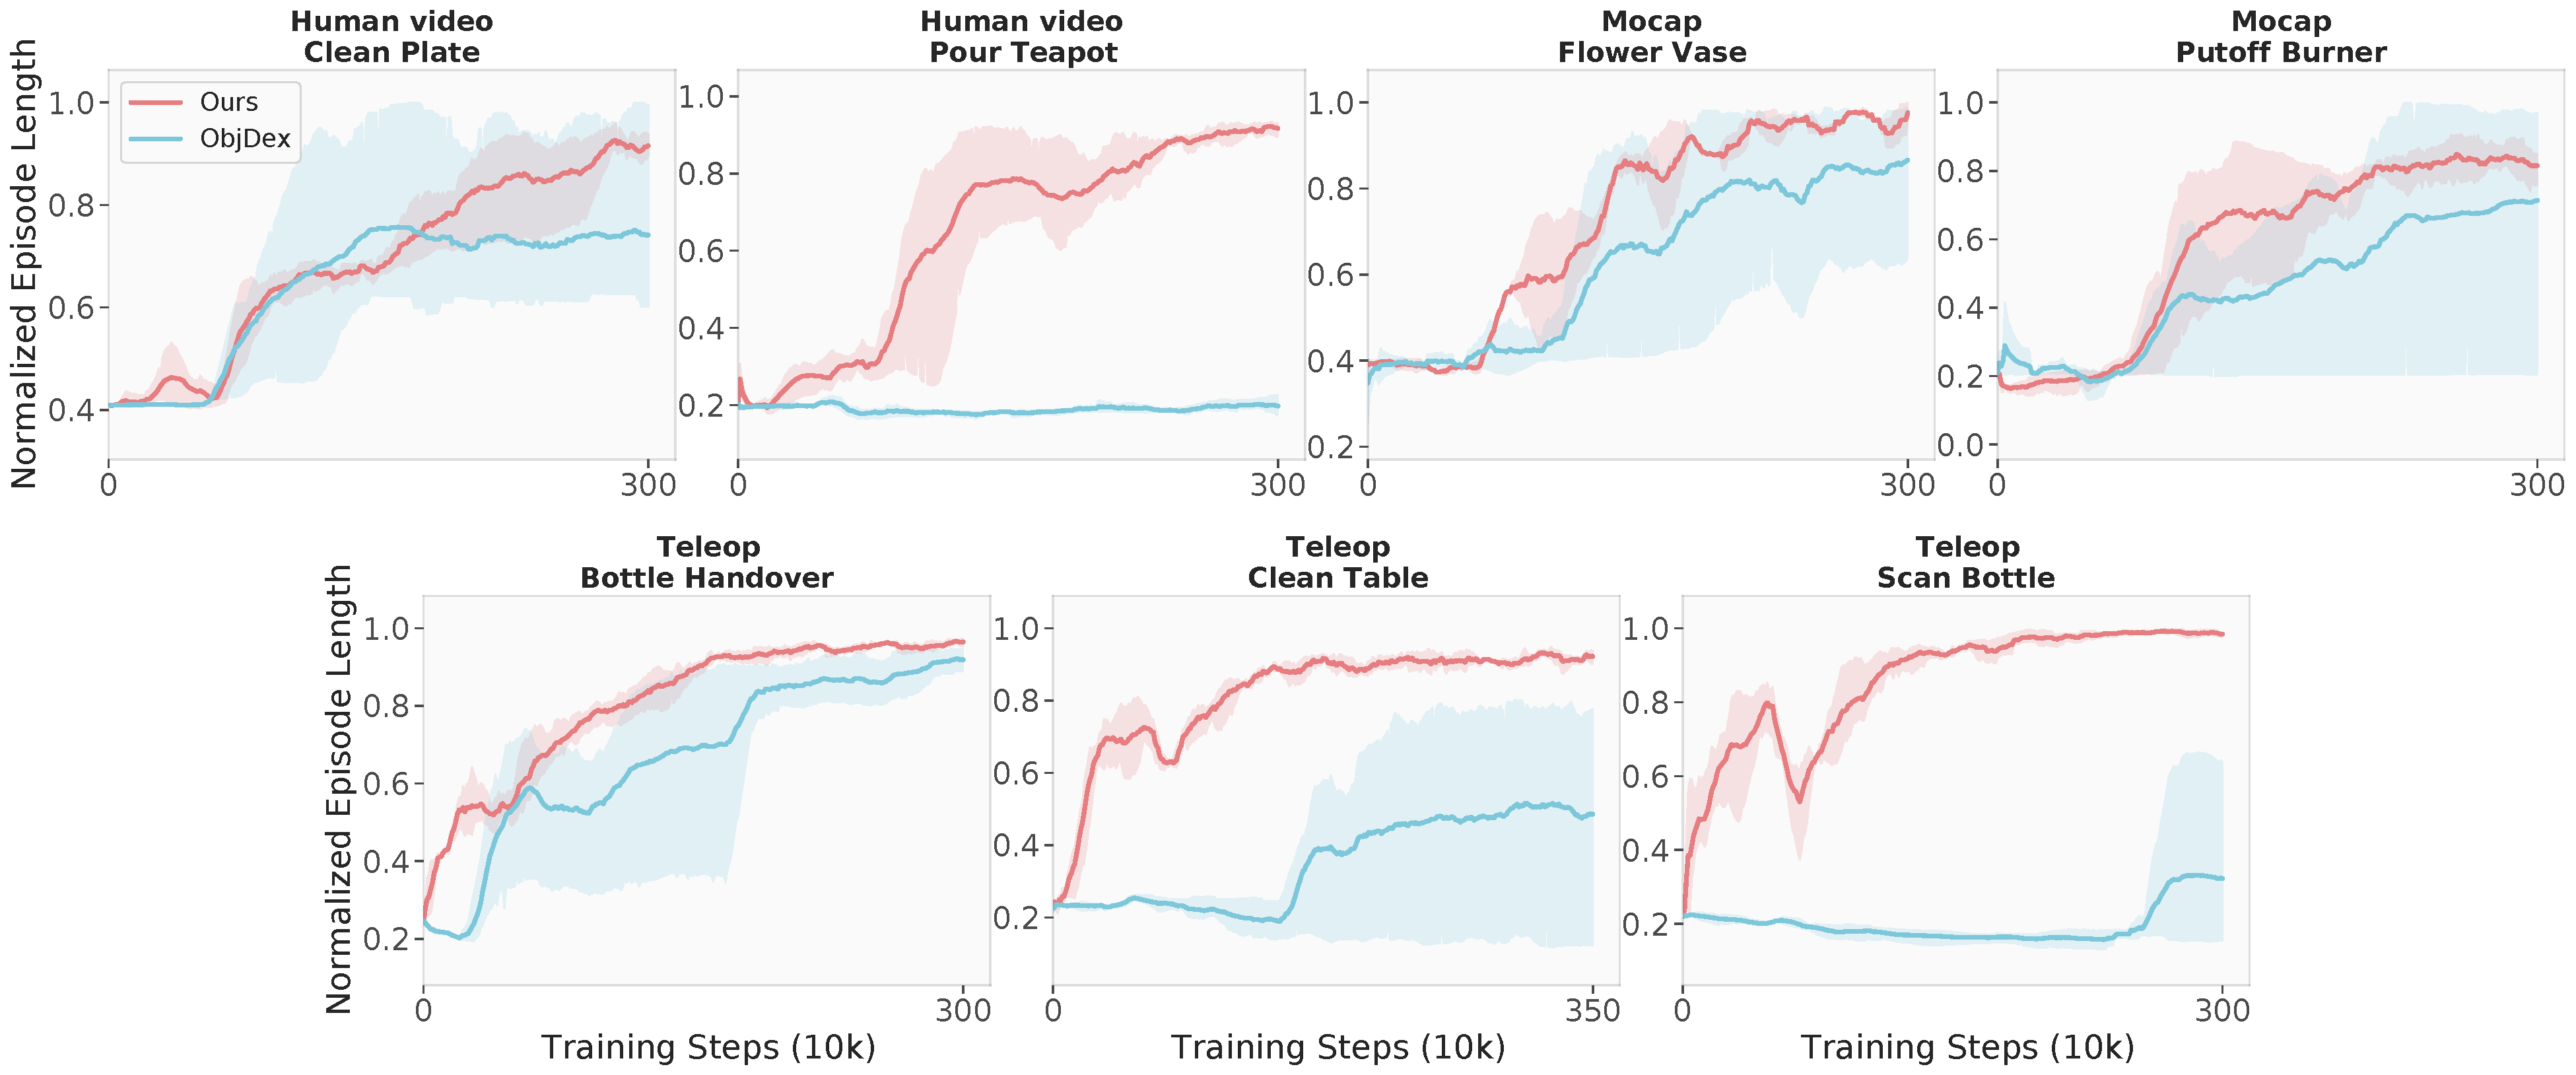
\includegraphics[width=1.0\linewidth]{figures/train_curve_new.pdf}
  \caption{ \textbf{The training curve of \ourshort.} The horizontal axis denotes the training steps, while the vertical axis represents the normalized task length successfully accomplished by the policy. \textit{Teleop} refers to one-shot human motion teleoperation in simulation, \textit{Human video} denotes trajectories extracted from video data, and \textit{Mocap} corresponds to motion derived from mocap datasets. \ourshort not only demonstrates the capability to accomplish diverse manipulation tasks originating from various forms of human motion, but also exhibits superior sample efficiency throughout training. All results are evaluated across 3 seeds. }
  \label{fig:train_curve}
\end{figure*}
We evaluate the training sample efficiency of \ourshort across seven tasks. The visualizations of simulation tasks are shown in Figure~\ref{fig:sim_vis}. For each task, the source of the one-shot human motion demonstration is indicated in the title of each sub-figure in Figure~\ref{fig:train_curve}. The vertical axis in the figure represents the proportion of the trajectory length successfully executed by the current policy relative to the total length of the trajectory. As demonstrated in Figure~\ref{fig:train_curve}, regardless of the origin of the human motion data, \ourshort reliably succeeds in converting human hand and arm actions into generalizable robot-executable behaviors.


Additionally, we compare training performances with ObjDex~\cite{chenobject}. ObjDex defines its reward based on the tracking of the object's joint movement, translations, and orientations. We re-implement this reward formulation within our own algorithmic framework. Figure~\ref{fig:train_curve} indicates that \ourshort exhibits superior performance relative to ObjDex across all tasks. In tasks such as \textit{Bottle Handover}, \textit{Flower Vase}, and \textit{Putoff Burner}, where interactions involve only a single object, ObjDex is able to complete the tasks; however, \ourshort can achieve higher sample efficiency during training. Furthermore, in more intricate tasks involving multi-object interactions, ObjDex consistently fails, irrespective of the type of human motion data provided. Owing to our object-centric distance chain, \ourshort is capable of robustly acquiring diverse manipulation skills even in long‑horizon, multi-object environments. Moreover, \ourshort demonstrates high sample efficiency and successfully learns policies in 3M training steps.


\begin{figure}[h]
  \centering
  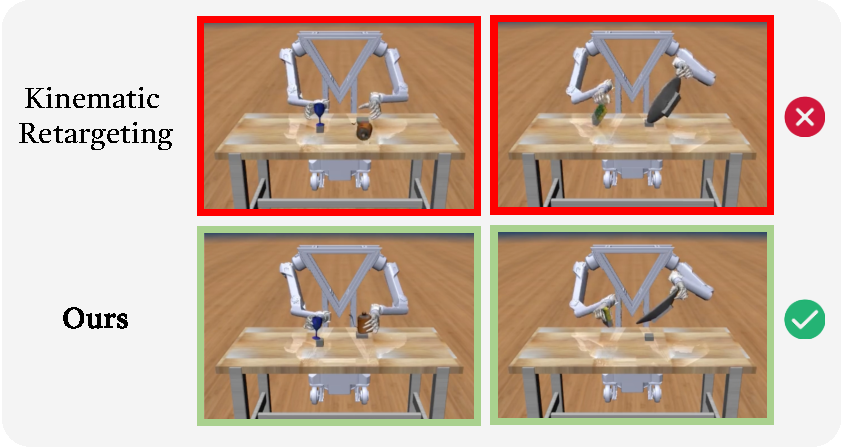
\includegraphics[width=1.0\linewidth]{figures/kinematics_pic.pdf}
  \caption{ \textbf{The comparison of kinematic retargeting and \ourshort.} The raw trajectories extracted from human videos and mocap data are insufficient to complete the task through mere kinematic retargeting. On the other hand, \ourshort not only learns to follow these reference trajectories but also masters the nuances of object interaction.}
  \label{fig:kinematics}
\end{figure}

\subsection{Comparison with Non-learning Approach}
In this section, we highlight the central role of reinforcement learning in equipping robots with adaptive policies and delineate the advantages it affords over non-learning approaches.

\begin{table}[h]
\centering
\caption{Comparison of \ourshort and kinematic retargeting.}
\label{table: compare_retarget}
\resizebox{0.5\textwidth}{!}{
\begin{tabular}{c|cc}
\toprule

\setlength{\tabcolsep}{10pt}
\begin{tabular}[c]{@{}c@{}} \multicolumn{1}{c}{\multirow{1}{*}{Tasks $\backslash$ Method}} \end{tabular}   & \multicolumn{1}{c}{\ourshort} & \multicolumn{1}{c}{kinematic retargeting} \\

\midrule

Video tasks & \ddbf{78.1}{15.0} & $0$ \\

Mocap tasks &	\ddbf{88.9}{6.7} & $0$ \\

\bottomrule
\end{tabular}
}
\end{table}


For human motion trajectories derived from mocap data and videos, we compare \ourshort with kinematic retargeting methods. Table~\ref{table: compare_retarget} indicates that while kinematic retargeting can map human hand motions to robotic counterparts, it fails to capture essential aspects such as object interactions and contact information. Moreover, the retargeting approaches cannot guarantee optimality. The snapshots of two approaches are visualized in \ref{table: compare_replay}. Hence, RL emerges as a crucial approach for refining robotic behaviors. It shapes the robot policies toward human-like motions and establishes physically plausible, context-appropriate object interactions.

\begin{table}[h]
\centering
\caption{Comparison of \ourshort and replay edited trajectories.}
\label{table: compare_replay}
\resizebox{0.4\textwidth}{!}{
\begin{tabular}{c|cc}
\toprule

\begin{tabular}[c]{@{}c@{}} \multicolumn{1}{c}{\multirow{1}{*}{Tasks $\backslash$ Method}} \end{tabular}   & \multicolumn{1}{c}{\ourshort} & \multicolumn{1}{c}{replay} \\

\midrule

Bottle Handover & \ddbf{91.9}{1.9} & \dd{52.2}{5.1}  \\

Place Drawer &	\ddbf{72.2}{5.1} & \dd{49.9}{5.8}  \\

\bottomrule
\end{tabular}
}
\end{table}

Regarding teleoperation data, we compare \ourshort with direct replay of edited trajectories. We evaluate both methods on two distinct tasks: a long-horizon task involving articulated object manipulation~(\textit{placedrawer}) and a contact-rich task~(\textit{handover}). For each task, the object's pose is randomized on the table, and each method is evaluated over 30 episodes. As demonstrated in Table~\ref{table: compare_replay}, due to the robot's dynamic configuration, directly executing edited actions does not guarantee task success when object positions change. In contrast, \ourshort, through RL training, learns residual actions that can adaptively adjust movements and enhance execution success rates. These results also highlight that \ourshort leveraging RL can effectively mitigate dynamic inconsistencies. 
\begin{figure*}[t]
  \centering
  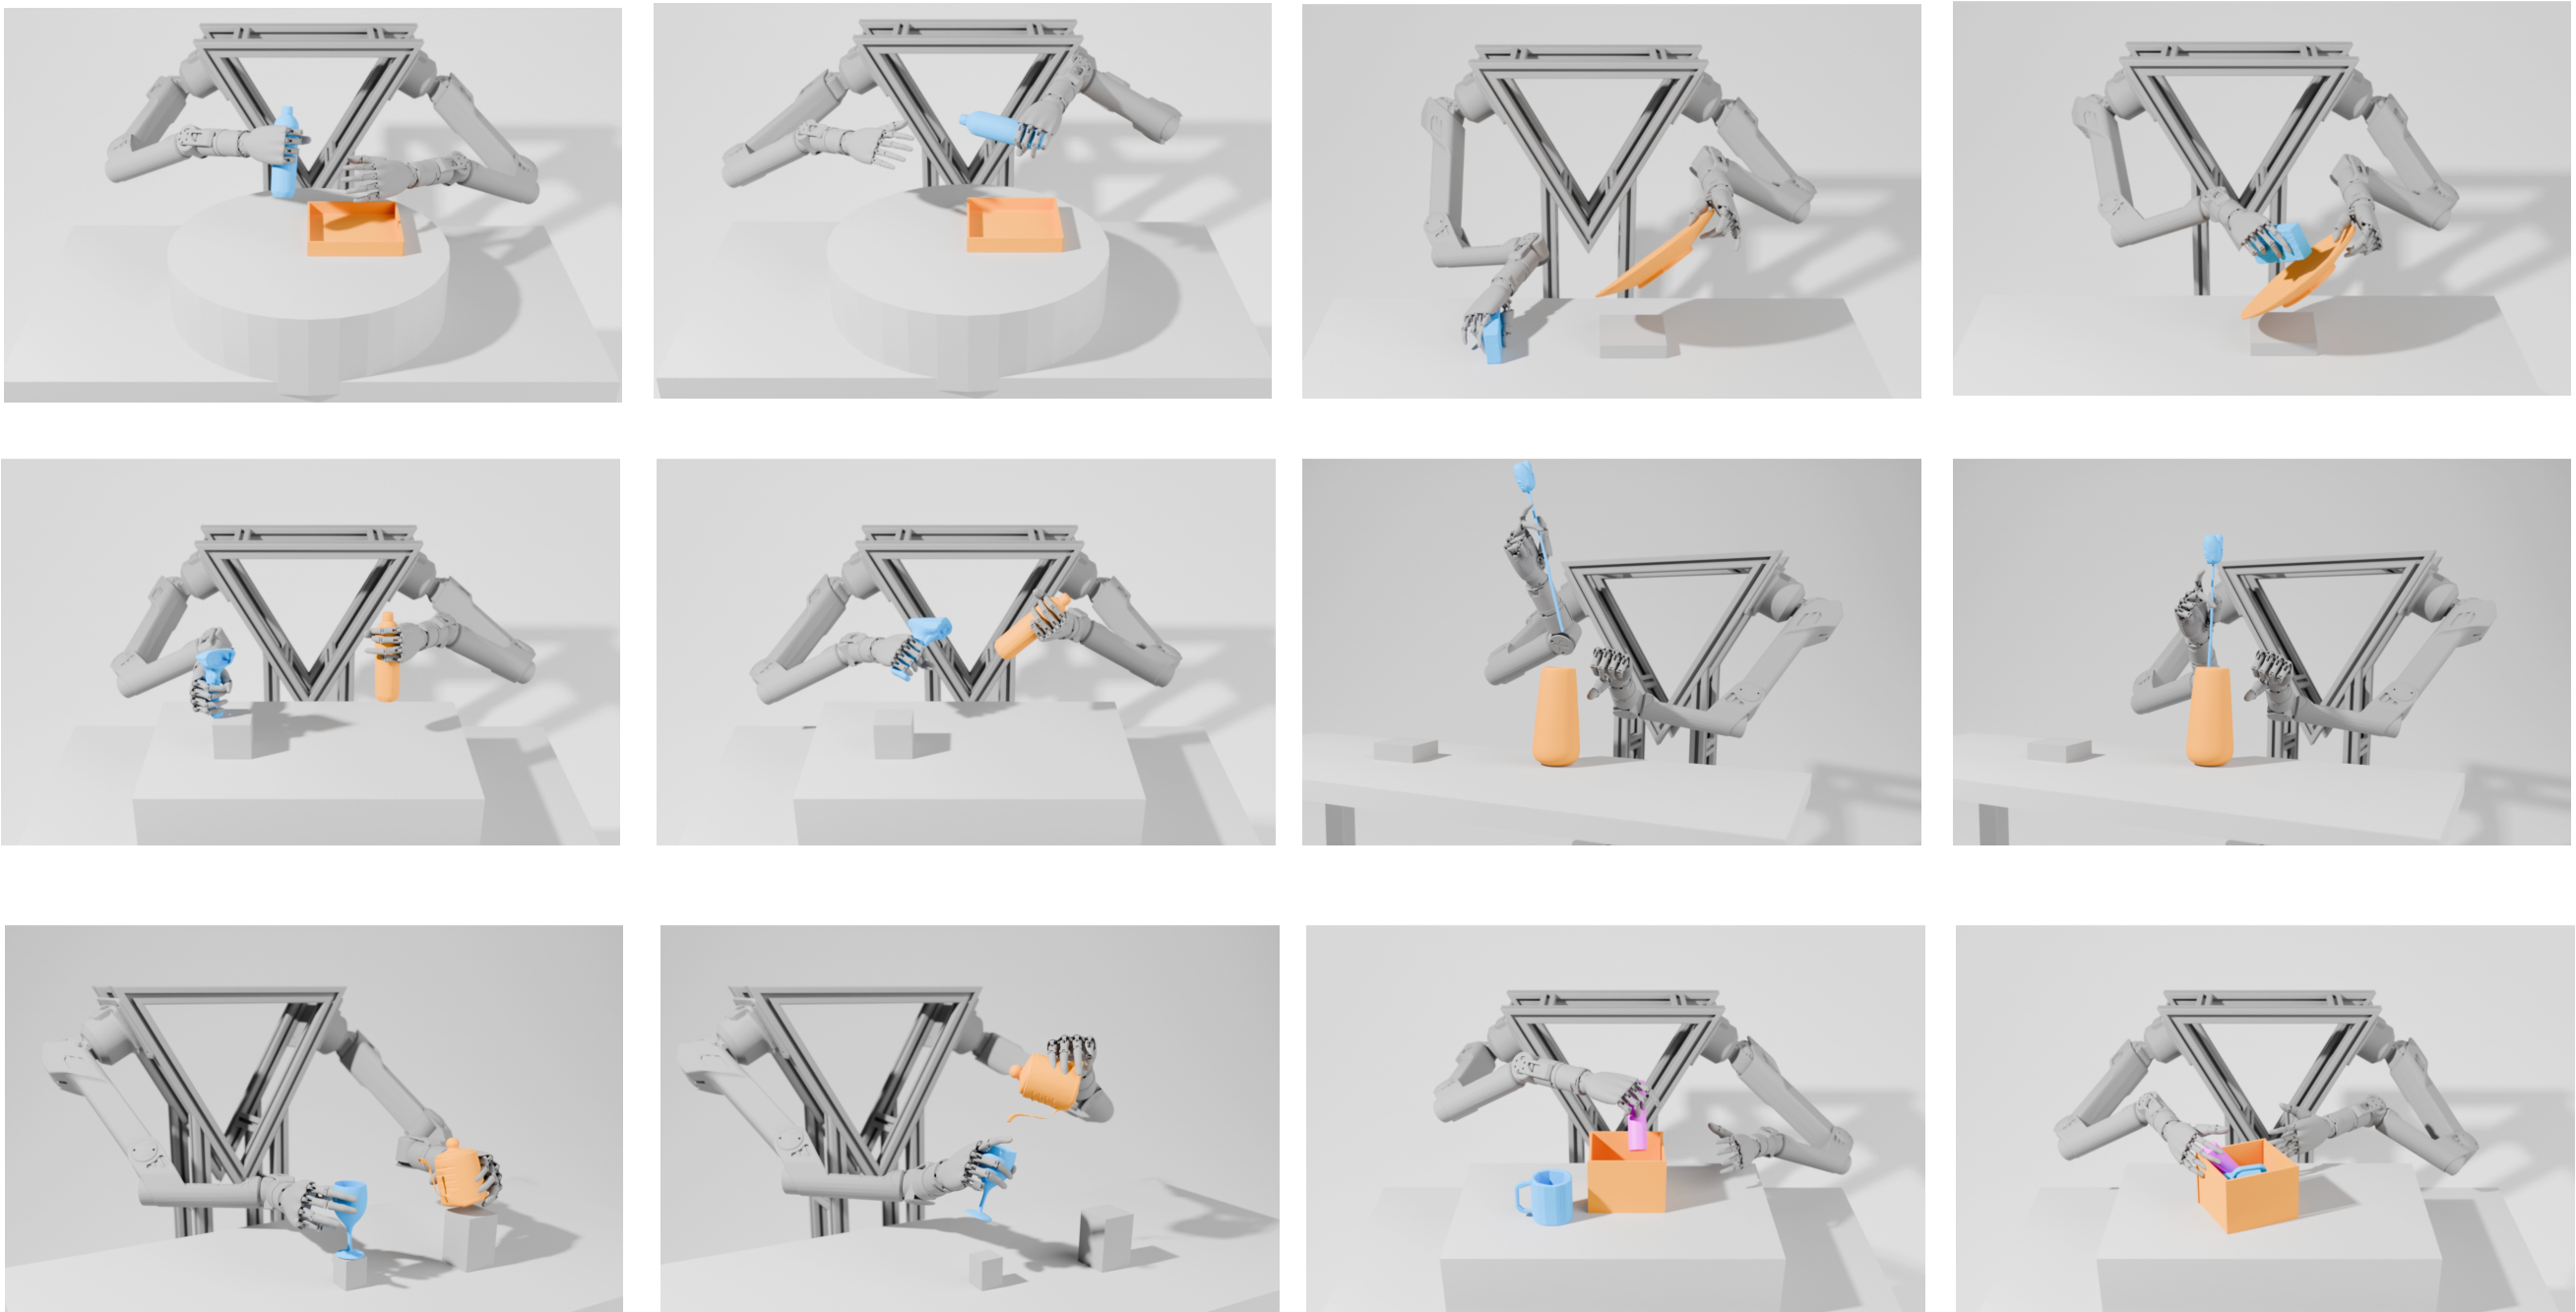
\includegraphics[width=1.0\linewidth]{figures/sim_vis_pic.pdf}
  \caption{ \textbf{Simulation training visualization.} We visualize the majority of the training tasks. Leveraging a single reference trajectory in conjunction with a general reward design, \ourshort can convert diverse human motion sources into robot feasible behaviors via RL training.}
  \label{fig:sim_vis}
\end{figure*}
\begin{figure}[h]
  \centering
  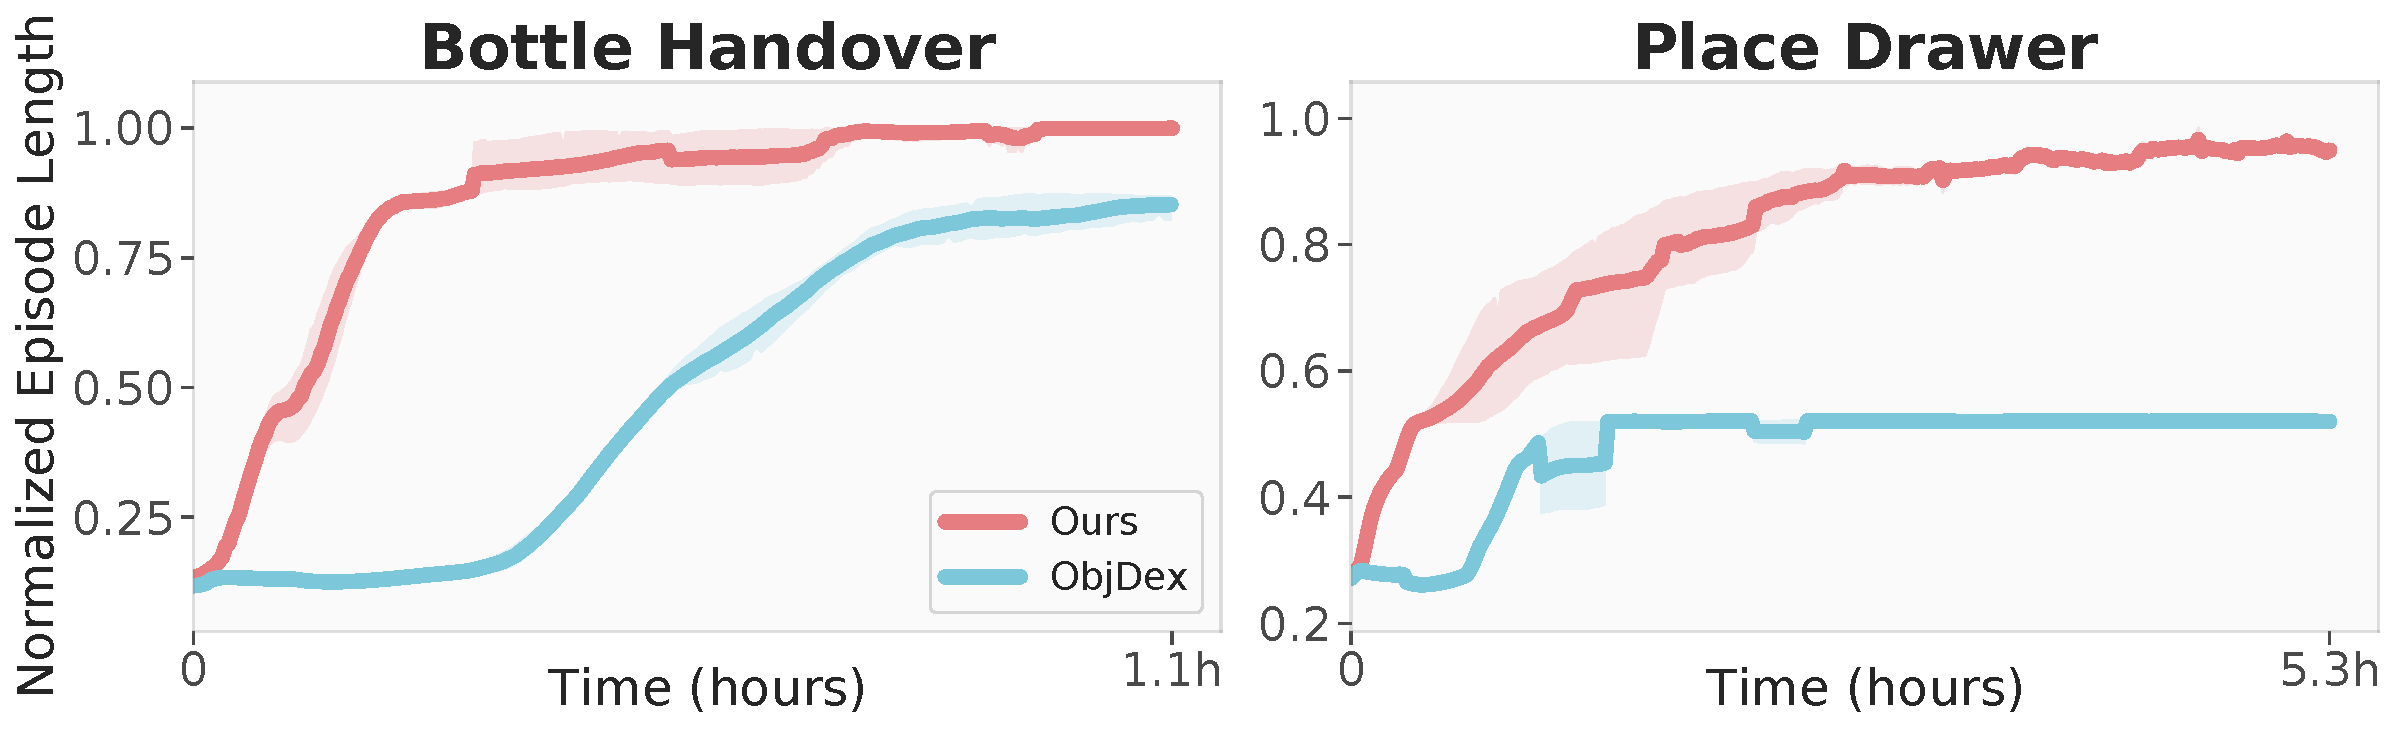
\includegraphics[width=1.0\linewidth]{figures/walltime_curves_pic.pdf}
  \caption{ \textbf{The wall-time training efficiency.} \ourshort also enjoys  high wall-time efficiency under parallel training. All results are evaluated across 3 seeds.}
  \label{fig:walltime}
\end{figure}
\subsection{Training wall-time}
We also leverage the MJX GPU parallel simulation~\cite{MJX} to instantiate the tasks and adopt the PPO algorithm~\cite{schulman2017proximal} for policy training. We adopt reward terms in line with DrM. As illustrated in Figure~\ref{fig:walltime}, \ourshort benefits from reduced wall-clock training time, and the reward formulation demonstrates cross-algorithm generality. Meanwhile, compared to the baseline method, \ourshort also attains higher sample efficiency and stronger asymptotic performance under PPO training.

\begin{figure*}[t]
  \centering
  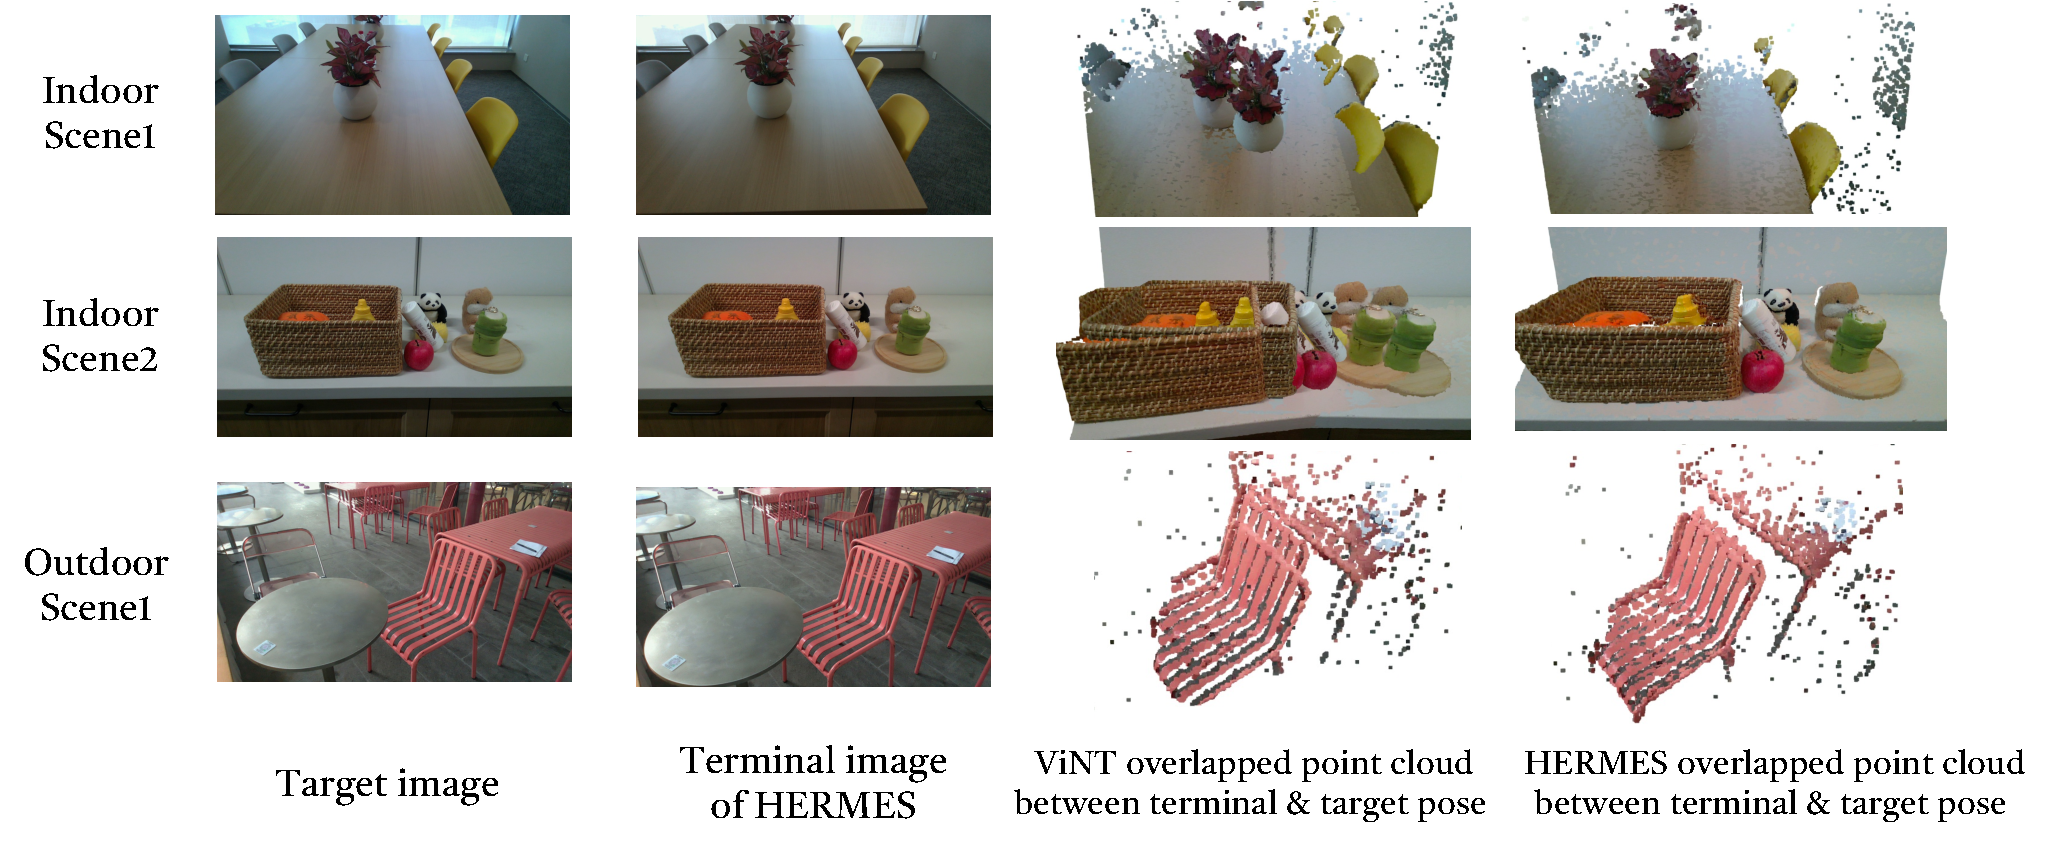
\includegraphics[width=1.0\linewidth]{figures/nav_result_pic.pdf}

  \caption{ \textbf{The visualization of navigation results.} The left two columns depict a comparison between the target image and the terminal image achieved by our method. The right two columns present the point clouds captured at the end of navigation by ViNT and \ourshort, compared against the point cloud of the target position. This figure illustrates that ViNT exhibits a noticeable mismatch between the captured and target point clouds at the end of navigation, whereas \ourshort achieves a close alignment, which demonstrates the high localization accuracy of our approach.}
  \label{fig:nav_result}
\end{figure*}



\subsection{Real-world Manipulation Evaluation}

\begin{table*}[t] \caption{Real-world manipulation  evaluation results. Across $6$ real-world bimanual dexterous manipulation tasks, \ourshort obtains $\mathbf{+54.5\%}$  performance gains on average. }
\label{table1: generalization}
\centering
\renewcommand\tabcolsep{4.0pt}
\renewcommand{\arraystretch}{1.2}
\begin{normalsize}
\resizebox{0.9\textwidth}{!}{
\begin{tabular}{c|cccccc|c}
\cline{2-6}
\toprule[0.3mm]
\begin{tabular}[c]{@{}c@{}}  \multicolumn{1}{c}{\multirow{1}{*}{Method  $\backslash$ Tasks}} \end{tabular} & Bottle Handover & Clean Table & Scan Bottle & Putoff Burner & Clean Plate & Pour Teapot &  \textbf{Average} \\
% Setting & \begin{tabular}[c]{@{}c@{}}Method $\backslash$ Tasks\end{tabular} & \begin{tabular}[c]{@{}c@{}}MW~(Medium 11) \end{tabular} & \begin{tabular}[c]{@{}c@{}}MW~(Hard 5) \end{tabular}   & \begin{tabular}[c]{@{}c@{}} MS~(Deformable 4) \end{tabular}  & \begin{tabular}[c]{@{}c@{}} DexArt~(4)  \end{tabular}  \\  \hline
\hline 
\begin{tabular}[c]{@{}c@{}} \ourshort  \end{tabular} & \best{66.7}  & \best{60.0} & \best{73.3}  & \best{66.7} & \best{66.7} & \best{73.3}   & \textcolor{lyydeepred}{\ddbf{67.8}{5.0}} \\
\begin{tabular}[c]{@{}c@{}} raw depth \end{tabular}  & $6.7$ & $0.0$  &  $0.0$  & $20.0$   &   $13.3$    & $40.0$   &   \dd{13.3}{15.2}   \\
\hline
\end{tabular}
}
% \end{tabular}

\end{normalsize}
\label{table:sim-results}
\vspace{-10pt}
\end{table*}


% \normalsize\textcolor{darkgreen}{$(+2.0\%)$}
After conducting DAgger training, we subsequently transfer the trained visual student policy to the real world in a zero-shot manner for most tasks. It should be noted that for the tasks \textit{pour teapot} and \textit{putoff burner}, the presence of substantial noise in the trajectory or transparent objects leads to excessively jittering motions, along with discrepancies between simulated and real-world object shapes. Consequently,  we additionally fine-tune the policy using 5 extra real-world trajectories collected via policy rollouts. 

Table~\ref{table:sim-results} presents the generalization performance of the policy evaluated across different object placements and poses, with each task assessed over 15 trials. As the baseline, we replace our depth-processing with raw depth inputs in the sim2real pipeline. \ourshort not only successfully achieves zero-shot transfer for diverse long-horizon or contact-rich bimanual dexterous manipulation tasks, but also surpasses the baseline by $\mathbf{+54.5}$\% in success rate. These experimental results substantiate \ourshort's capability to effectively bridge both visual and dynamic gaps, enabling successful sim2real transfer and demonstrating intricate manipulation skills. Moreover, for the two tasks involving fine-tuning with real-world rollout trajectories, owing to the reduced visual discrepancy achieved by \ourshort, the trained policy exhibits enhanced generalization capabilities compared to the raw depth baseline. 


\subsection{The Effectiveness of Closed-loop PnP}

In terms of the navigation experiments, we first evaluate the localization errors of the ViNT model augmented with our proposed closed-loop PnP localization algorithm. We conduct experiments in two indoor and one outdoor scenarios, including two long-horizon navigation tasks. Table~\ref{table:nav_error} reports the computed localization errors in both translational distance and orientation. These errors are derived by solving the PnP problem and subsequently calculating the relative pose differences between the terminal pose and the target pose within a shared reference frame. As shown in Table~\ref{table:nav_error}, incorporating our proposed approach significantly reduces localization errors, whereas ViNT suffers from substantial instability in localization accuracy. Additionally, we visualize the RGB images and corresponding point clouds of the stopping positions for both baselines and \ourshort. Figure~\ref{fig:nav_result} demonstrates that \ourshort not only achieves semantic alignment of RGB images but also accurately matches the point clouds with the target position due to improved localization precision. The experimental results presented in Figure~\ref{fig:nav_result} and Table~\ref{table:nav_error} highlight that current general navigation models, despite their ability to broadly match the goal image, exhibit large localization discrepancies, rendering them unsuitable for downstream visuomotor manipulation tasks. In contrast, through employing our simple yet robust closed-loop PnP localization algorithm, \ourshort not only successfully addresses the low precision of the mobile robot base, but also achieves small localization errors.


\begin{table}[ht]
\centering
\caption{The results of navigation localization error.}
\label{table:nav_error}
\resizebox{0.48\textwidth}{!}{
\begin{tabular}{l|cc|cc}
\toprule
\begin{tabular}[c]{@{}c@{}} \multicolumn{1}{c}{\multirow{2}{*}{Method  $\backslash$ Tasks}} \end{tabular} & \multicolumn{2}{c|}{\textbf{\ourshort}} & \multicolumn{2}{c}{\textbf{ViNT}}  \\
& \small dist error~(cm) & \small ori error~($^\circ$)  &\small dist error~(cm) &\small ori error~($^\circ$)  \\
\midrule
indoor scene1 & \blueddbf{2.4}{0.5} & \blueddbf{1.79}{1.12} & \dd{18}{11.3} & \dd{2.57}{1.98}  \\
indoor scene2 & \blueddbf{1.3}{0.5} & \blueddbf{0.57}{0.57}  & \dd{7.3}{3.1} & \dd{3.66}{1.91} \\
outdoor scene1 & \blueddbf{3.2}{1.8} & \blueddbf{1.67}{1.84}  & \dd{12.9}{7.4} & \blueddbf{1.63}{1.31} \\

\bottomrule
\end{tabular}}

\end{table}





\subsection{The Localization Ability of Closed-loop PnP in the Textureless Scenario}
\begin{figure}[h]
  \centering
  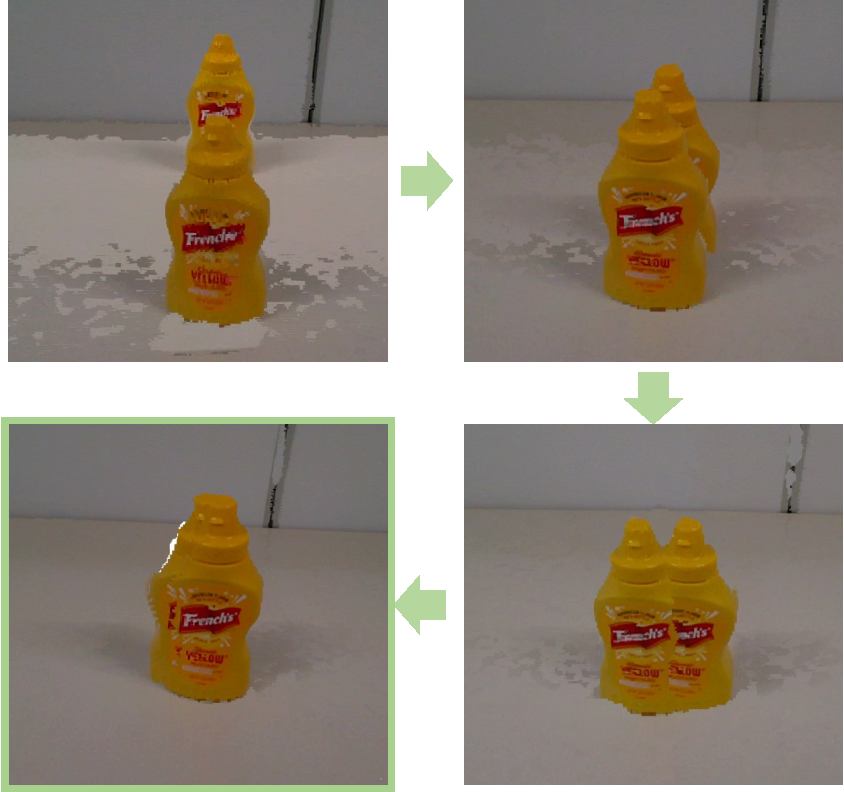
\includegraphics[width=0.9\linewidth]{figures/plain_pic.pdf}
  \caption{ \textbf{The localization ability of \ourshort in textureless scenarios.} Even in environments with sparse visual features, \ourshort remains capable of executing fine-grained positional adjustments and achieving precise localization through the closed-loop PnP mechanism.}
  \label{fig:plain}
\end{figure}
We also compare the localization performance of RTAB-MAP~\cite{Labb__2018}, a popular RGBD-based visual SLAM approach, against \ourshort in the textureless scenario. Previous studies have shown that RGBD-based SLAM methods struggle to accurately localize in textureless environments since it is hard to track visual features in these scenes~\cite{Labb__2018,Campos_2021,s19102251}. As shown in Table~\ref{table: nav_textureless}, RTAB-MAP fails to accomplish the task while our approach consistently achieves precise localization even under such challenging conditions. The point clouds of iterative refinement processes of closed-loop PnP are shown in Figure~\ref{fig:plain}.


\begin{table}[h]
\centering
\caption{Comparison of \ourshort and RTAB-MAP in the textureless scenario.}
\label{table: nav_textureless}
\resizebox{0.45\textwidth}{!}{
\begin{tabular}{c|cc}
\toprule

\begin{tabular}[c]{@{}c@{}} \multicolumn{1}{c}{\multirow{1}{*}{Method $\backslash$ Error}} \end{tabular}   & \multicolumn{1}{c}{dist error~(cm)} & \multicolumn{1}{c}{ori error~($^\circ$)} \\

\midrule

RTAB-MAP & - & -  \\

\ourshort &	\ddbf{1.26}{1.25} & \ddbf{2.06}{1.50}  \\

\hline
\end{tabular}
}
\end{table}

\begin{figure}[h]
  \centering
  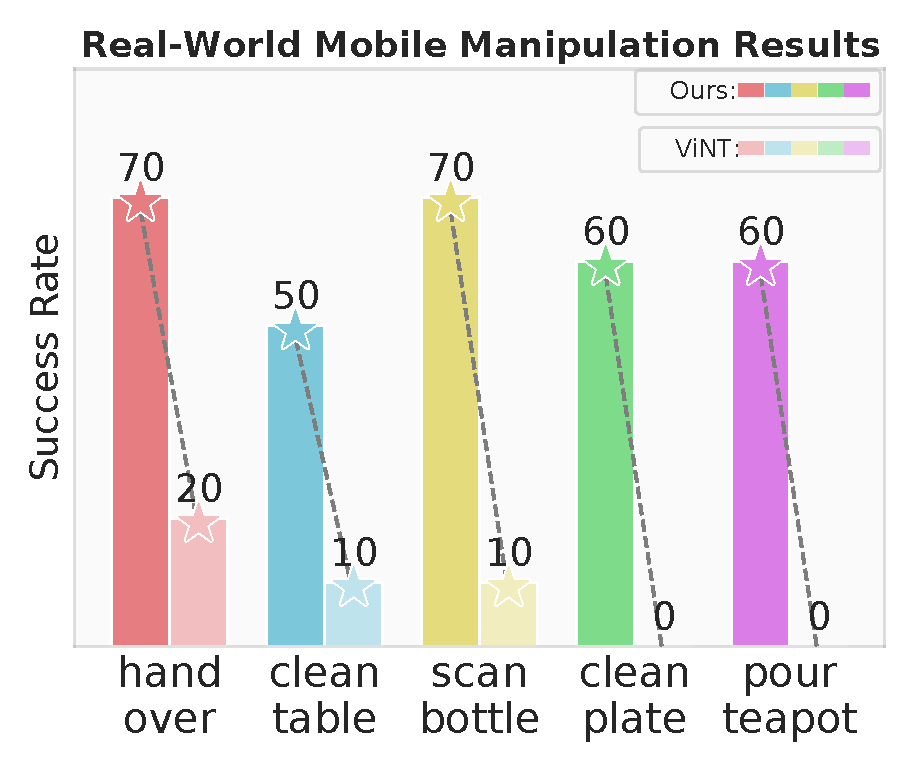
\includegraphics[width=1.0\linewidth]{figures/manipulation_bar_pic.pdf}
  \vspace{-15pt}
  \caption{ \textbf{Real-world mobile manipulation results.} Dark-colored bars correspond to \ourshort, whereas the light-colored bars correspond to only using ViNT. \ourshort is capable of performing a wide array of complex mobile bimanual dexterous manipulation tasks. In contrast, when relying solely on ViNT for localization, the trained manipulation policy fails to complete the tasks. } 
  \label{fig:mani_bar}
\end{figure}
\subsection{Mobile Manipulation Evaluation}
To evaluate the mobile manipulation ability of \ourshort, we integrate the entire pipeline across all tasks. Each trained policy is tested over 10 runs. As illustrated in Figure~\ref{fig:mani_bar}, \ourshort demonstrates strong real‑world navigation, precise localization, and dexterous manipulation capabilities. We also apply the identical manipulation policy equipped with ViNT as a baseline. Figure~\ref{fig:mani_bar} reveals that, without closed-loop PnP localization, the policy cannot generalize or successfully complete tasks when faced with significant positional and rotational shifts. Conversely, \ourshort achieves a notable $\mathbf{+54.0}$\% improvement in manipulation success rate compared to pure ViNT. These findings underscore that closed-loop PnP localization is the essential bridge linking navigation and manipulation, enabling both modules to synergize for enhanced performance.